\section{Results}
Localisation results.\\

%Results when the goal is [ 20 120 ].\\
\subsection{Results of a run in the test arena}
Here the results, of a run in the test arena with a random initial position and a goal in [20, 120], will be shown.
Figure \ref{ResultDriveFig1} shows how the robot initially tries to find its own location, using the particle filter. The number of particles is 200. It drives towards the farthest point read by the LIDAR while analysing its surroundings. In figure \ref{ResultDriveFig1:sub5} we see that the probability of a particle is over the threshold of 70\%, so the robots starts to plan its way towards the goal, using A*. 
\begin{figure}[H]
\centering
\begin{subfigure}{.5\textwidth}
  \centering
  \includegraphics[width=.8\linewidth]{billeder/Results/1.png}
  \caption{Step 1}
  \label{ResultDriveFig1:sub1}
\end{subfigure}%
\begin{subfigure}{.5\textwidth}
  \centering
  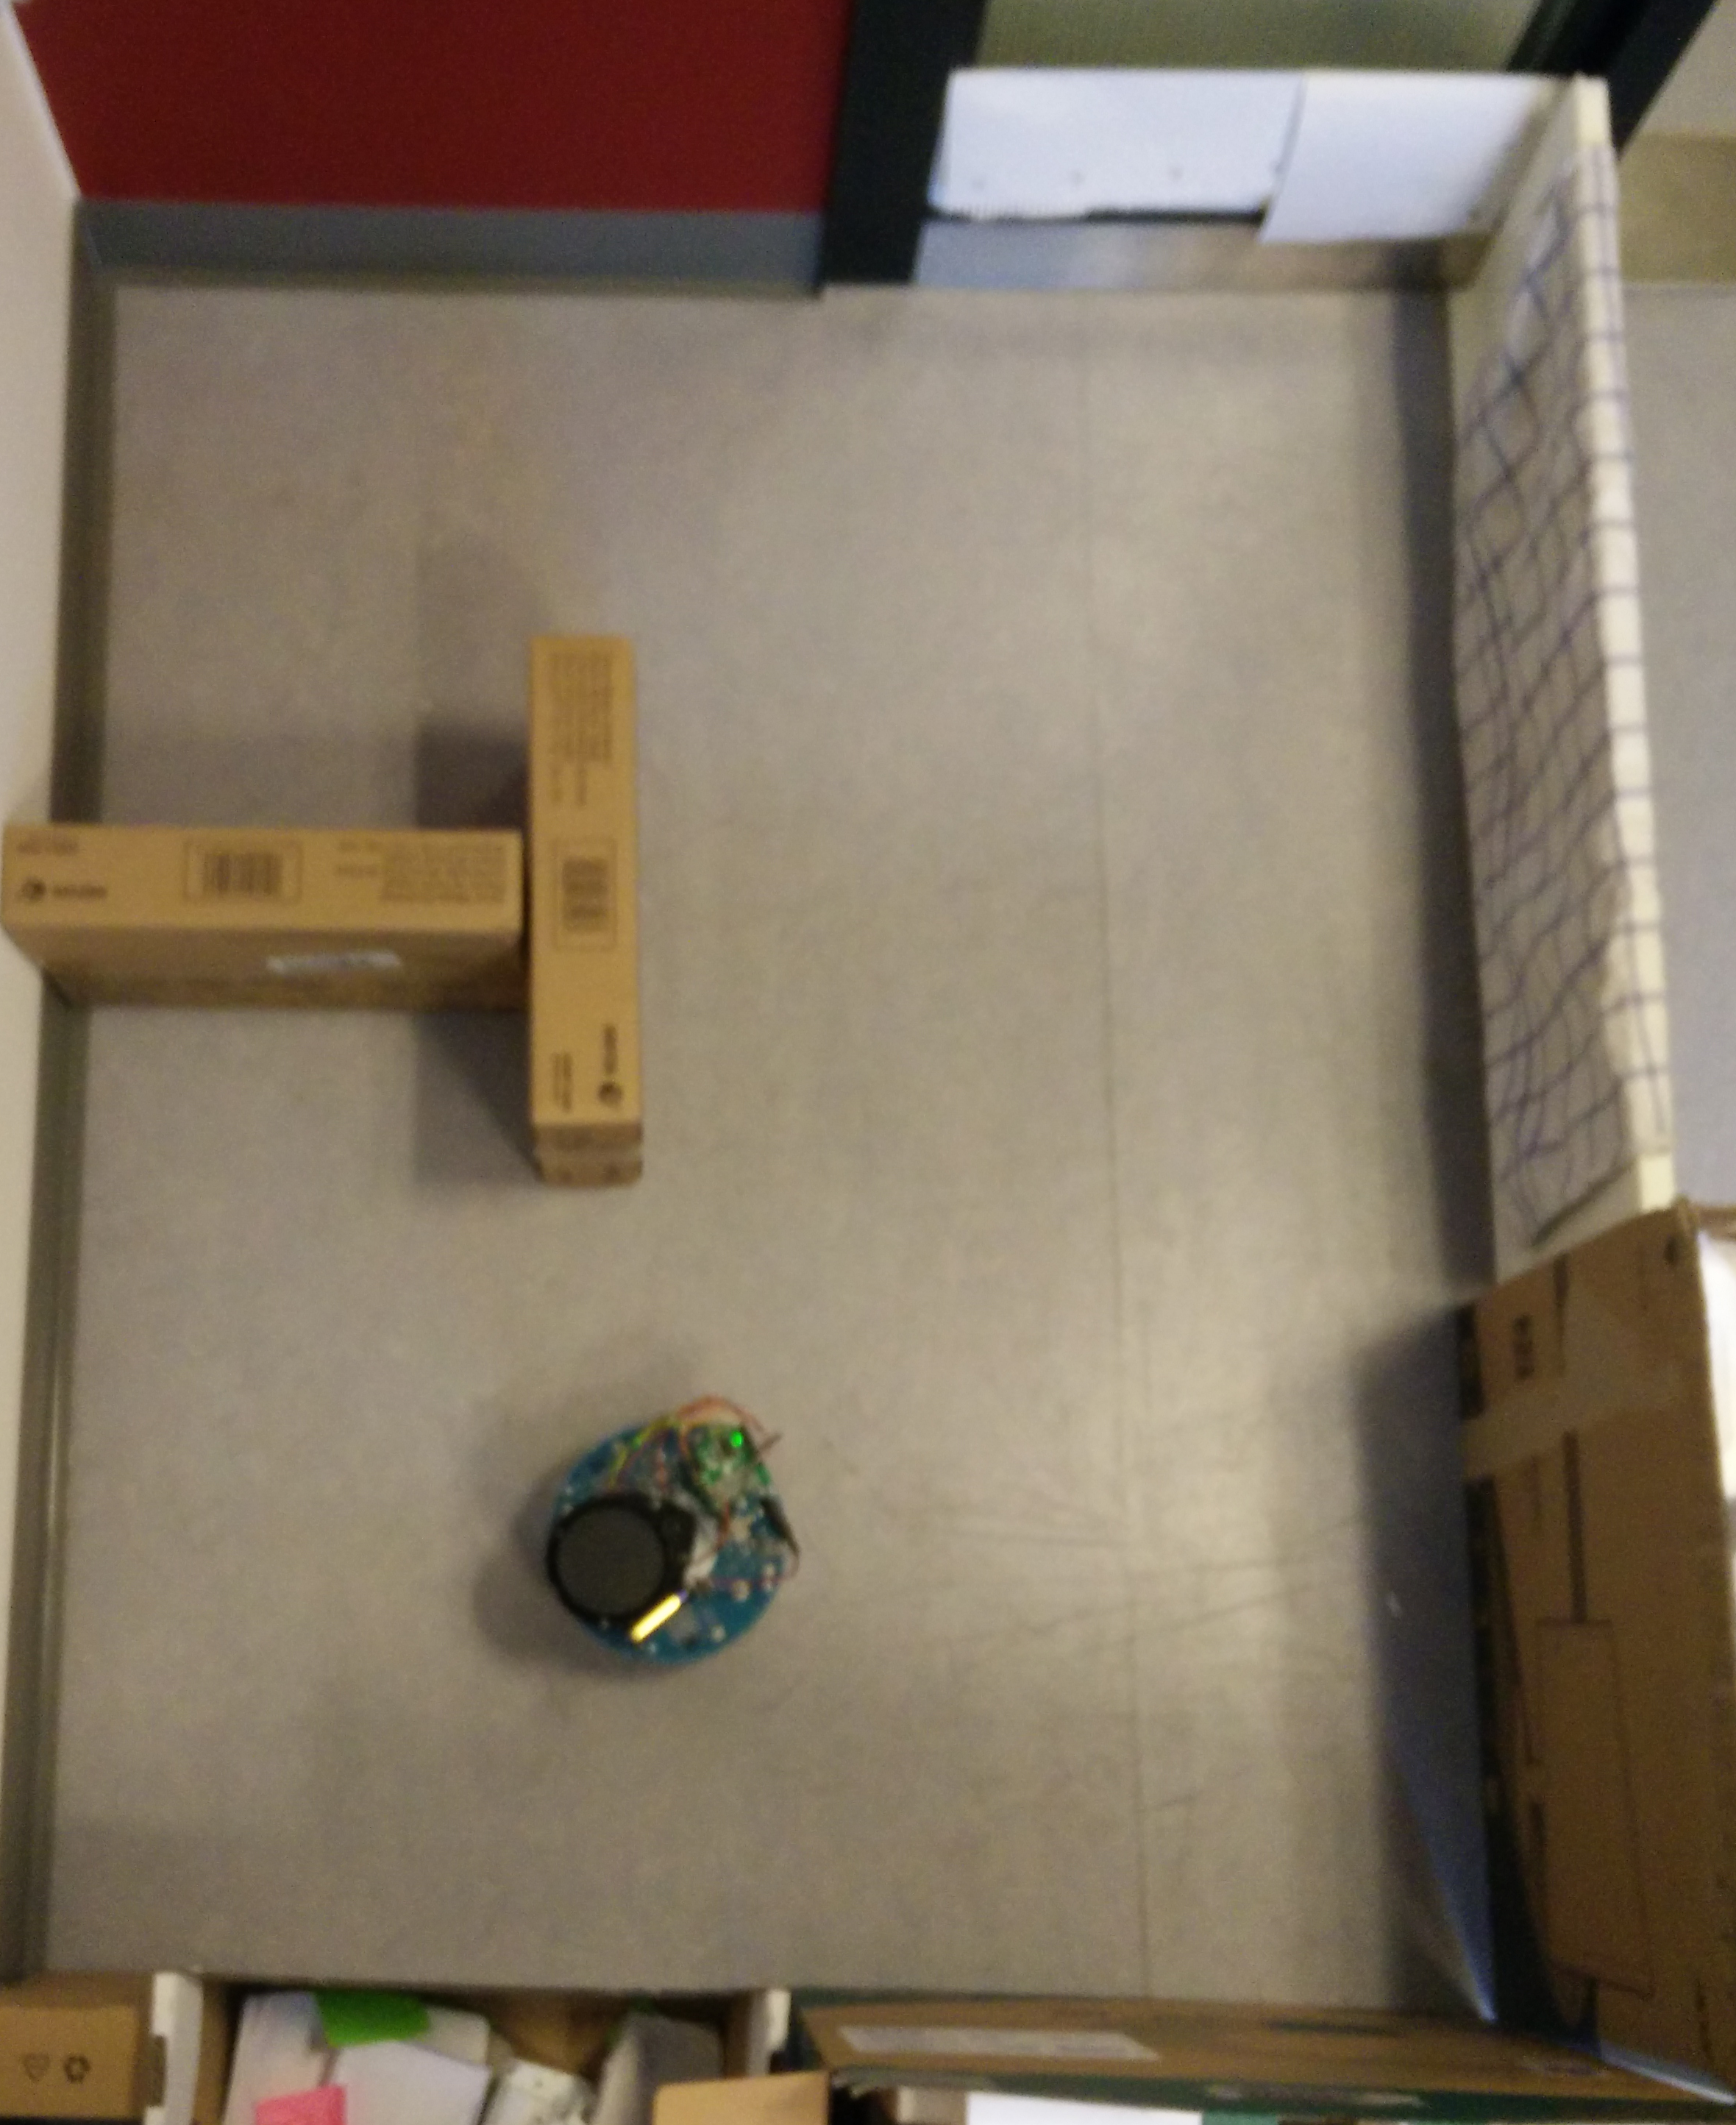
\includegraphics[width=.7\linewidth]{billeder/Results/real1.png}
  \caption{Step 1}
  \label{ResultDriveFig1:sub2}
\end{subfigure}
\begin{subfigure}{.5\textwidth}
  \centering
  \includegraphics[width=.8\linewidth]{billeder/Results/3.png}
  \caption{Step 3}
  \label{ResultDriveFig1:sub3}
\end{subfigure}%
\begin{subfigure}{.5\textwidth}
  \centering
  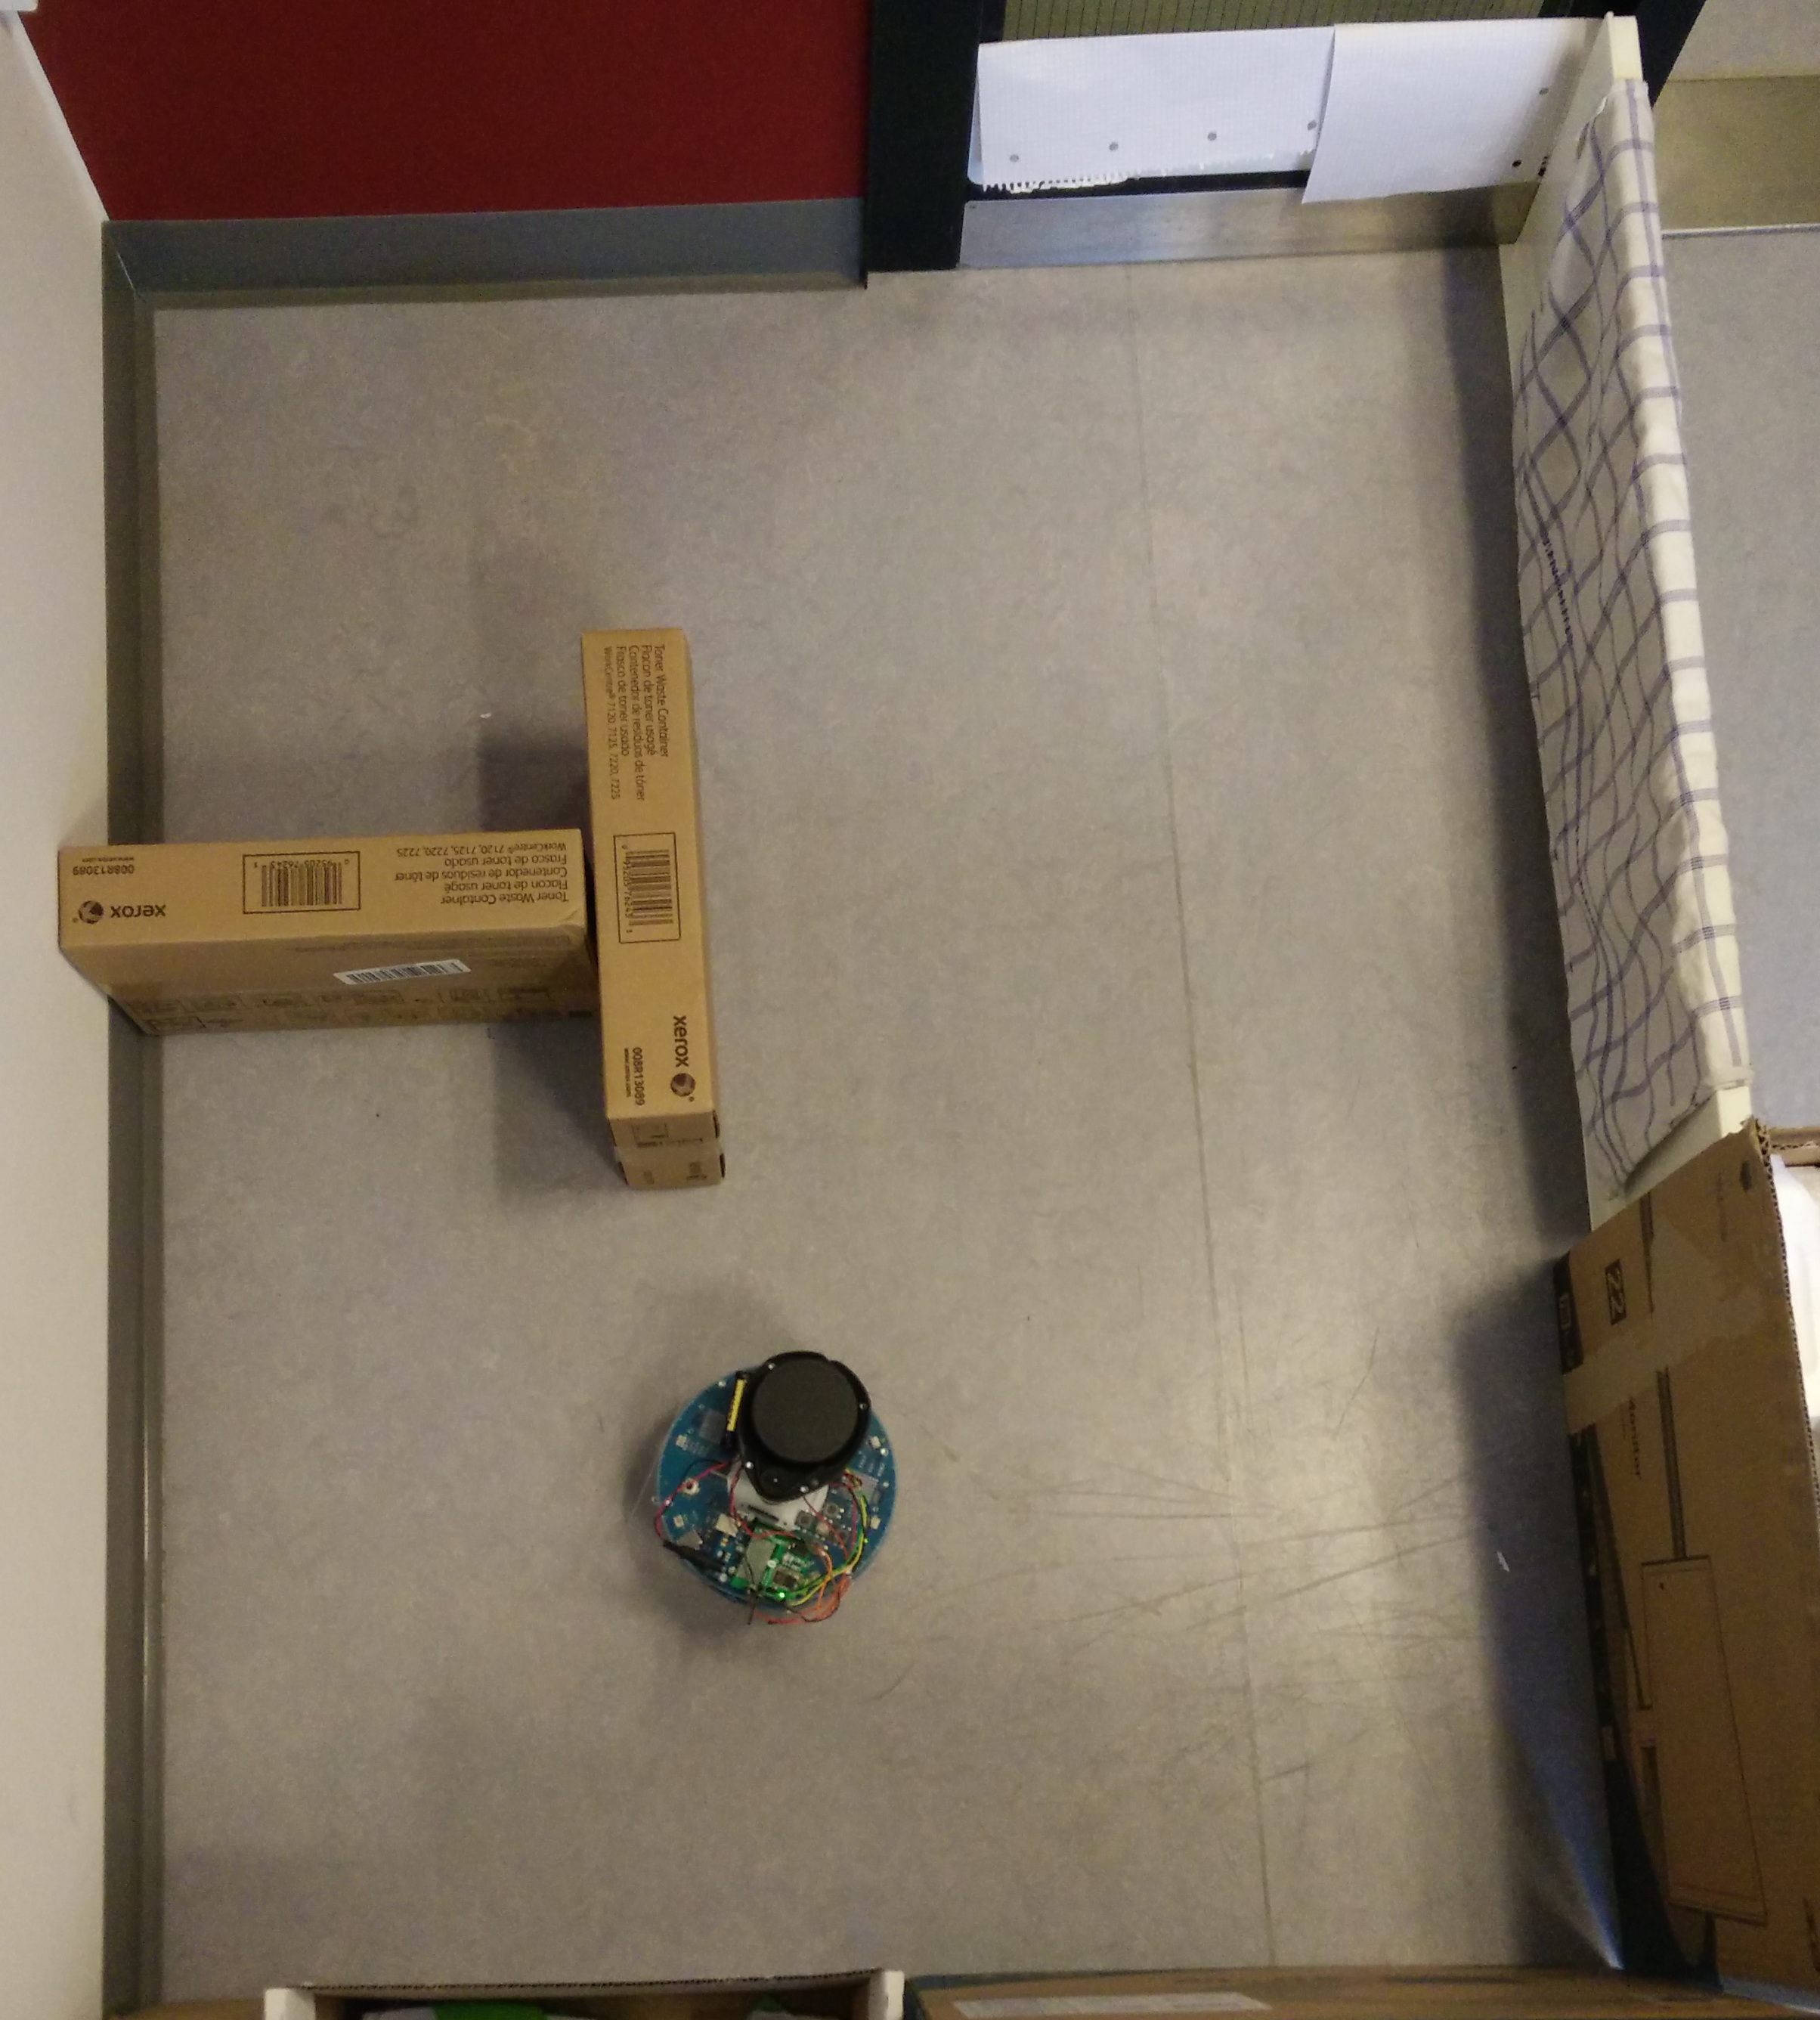
\includegraphics[width=.7\linewidth]{billeder/Results/real3.png}
  \caption{Step 3}
  \label{ResultDriveFig1:sub4}
\end{subfigure}
\begin{subfigure}{.5\textwidth}
  \centering
  \includegraphics[width=.8\linewidth]{billeder/Results/5.png}
  \caption{Step 5}
  \label{ResultDriveFig1:sub5}
\end{subfigure}%
\begin{subfigure}{.5\textwidth}
  \centering
  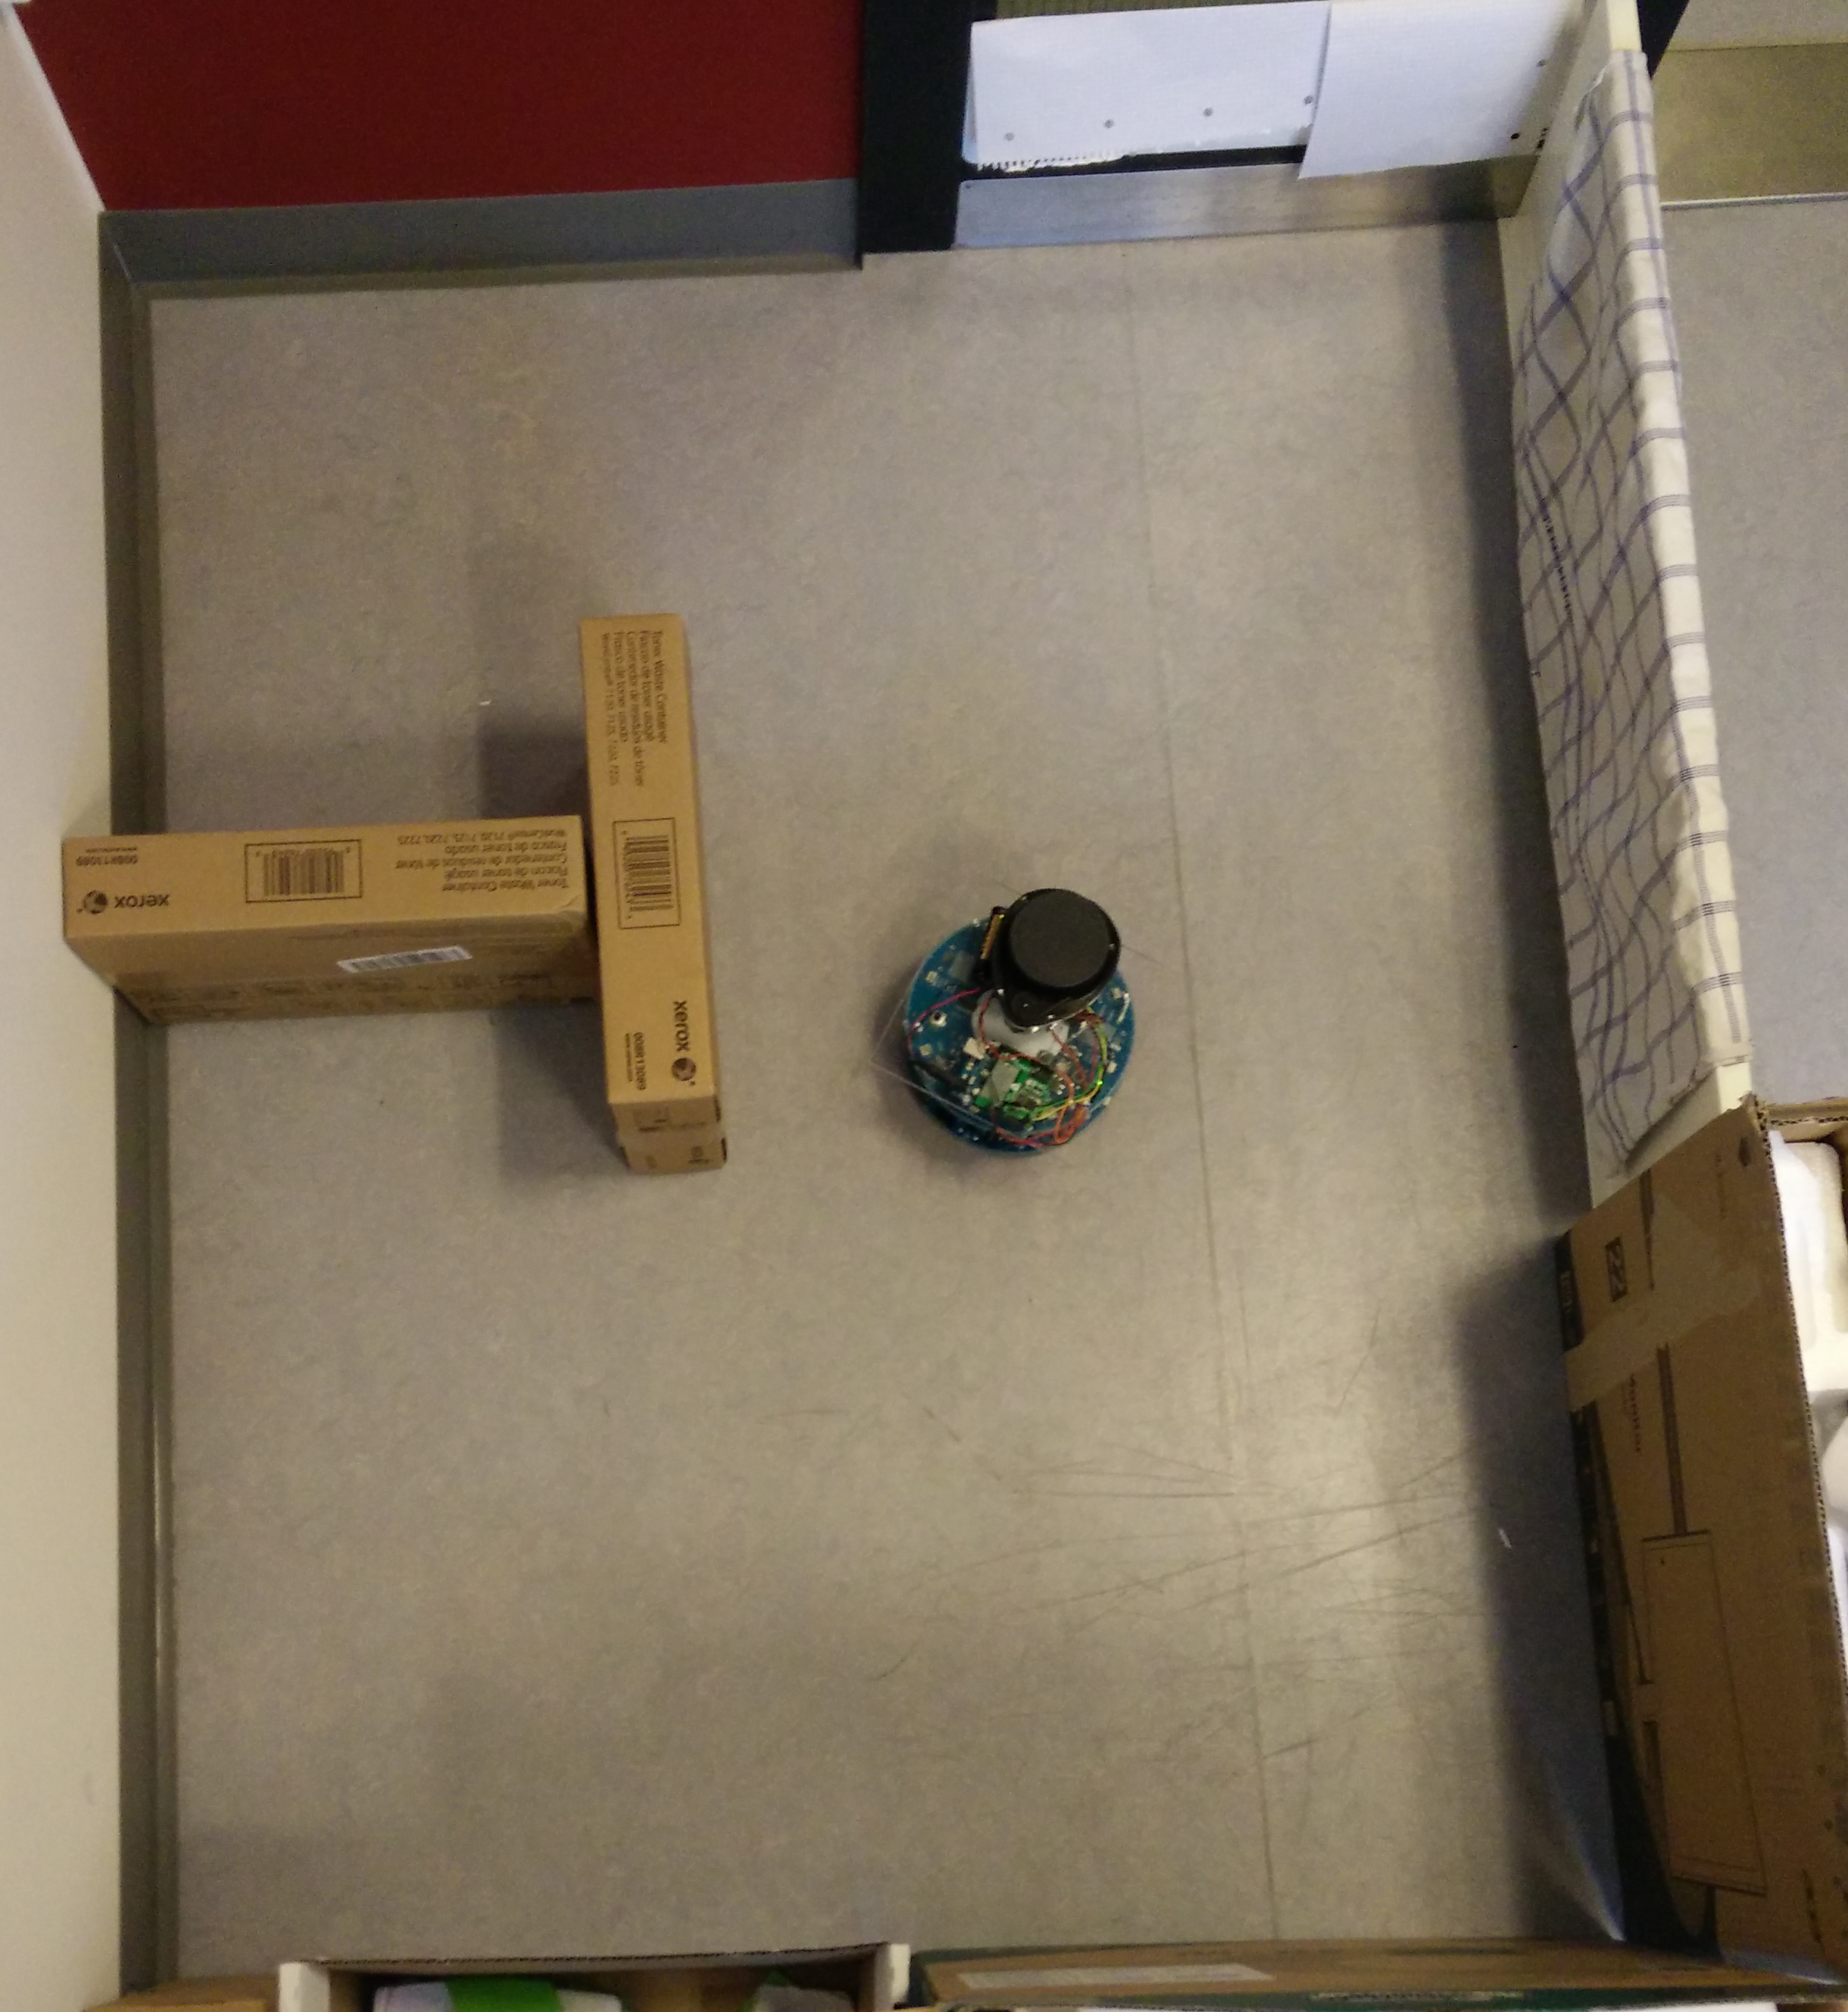
\includegraphics[width=.7\linewidth]{billeder/Results/real5.png}
  \caption{Step 5}
  \label{ResultDriveFig1:sub6}
\end{subfigure}
\caption{The robot tries to find its location.}
\label{ResultDriveFig1}
\end{figure}
Figure \ref{ResultDriveFig2} shows the robot trying to make it towards the points of the plan. The point the robot is aiming for is marked by a blue '+' on the particle filter map. The robot has to be within  5 cm of the point to believe that it is in the correct position.
\begin{figure}[H]
\centering
\begin{subfigure}{.5\textwidth}
  \centering
  \includegraphics[width=.8\linewidth]{billeder/Results/7.png}
  \caption{Step 7}
  \label{ResultDriveFig2:sub1}
\end{subfigure}%
\begin{subfigure}{.5\textwidth}
  \centering
  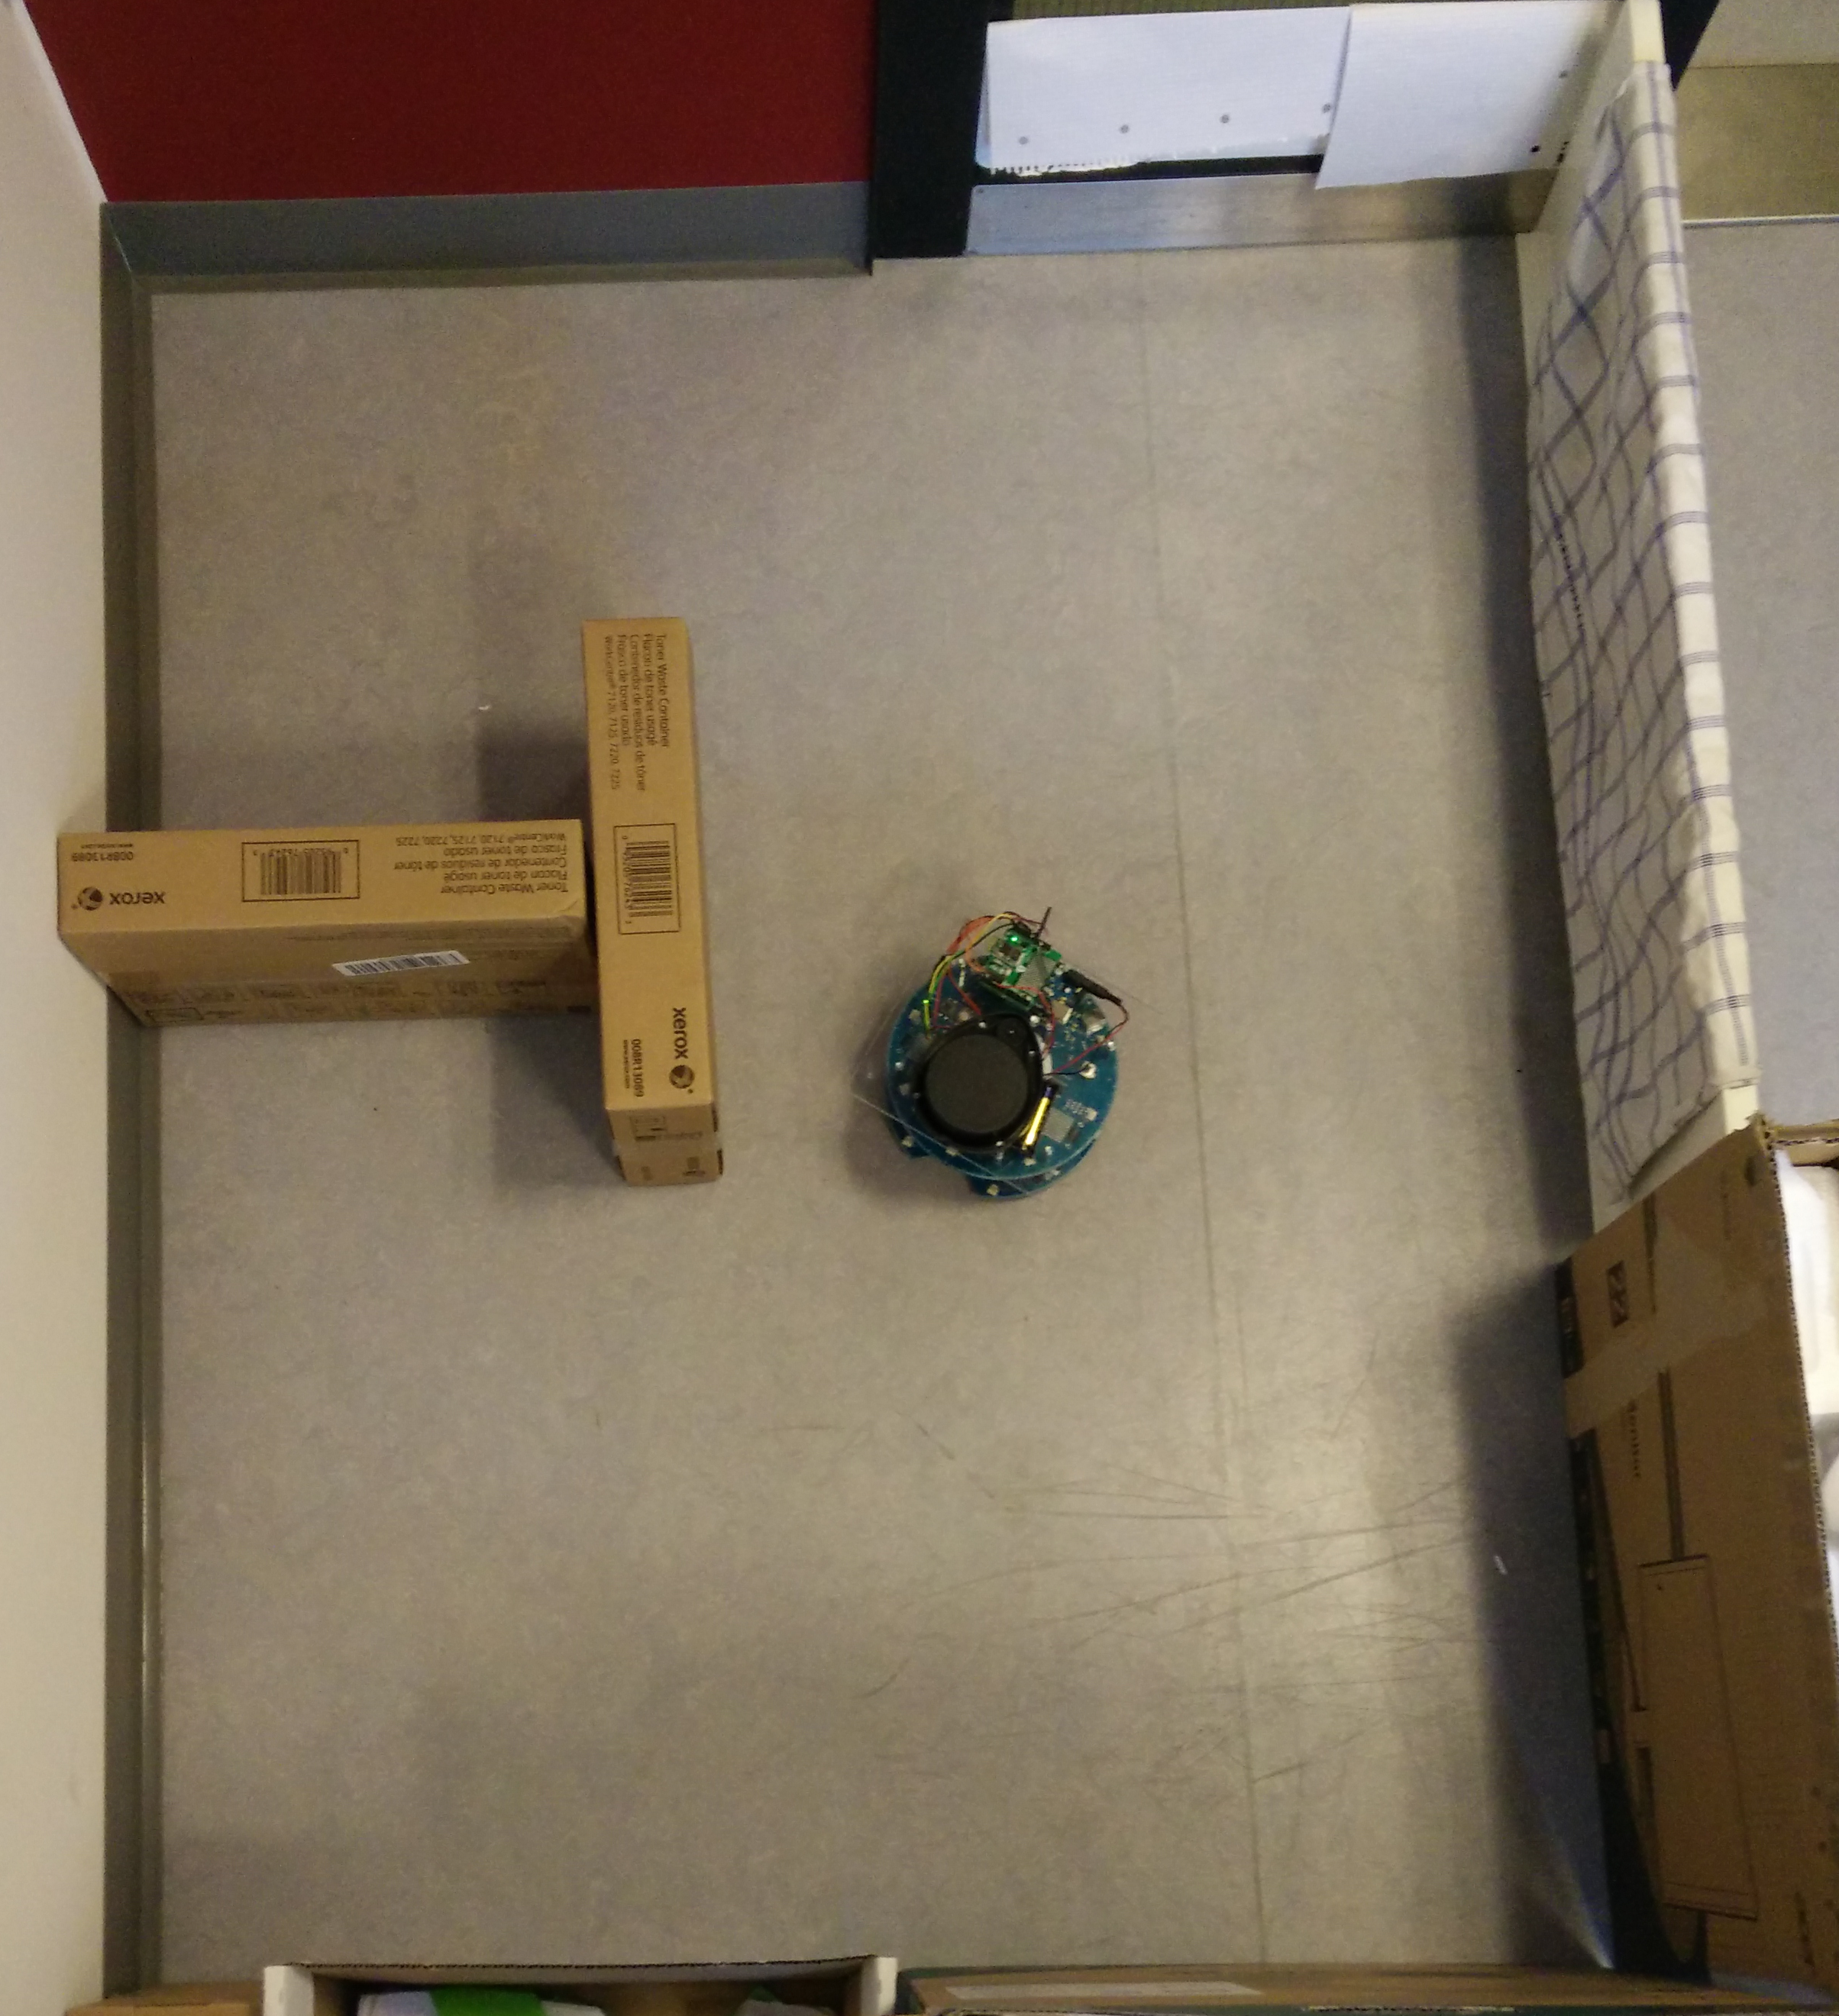
\includegraphics[width=.7\linewidth]{billeder/Results/real7.png}
  \caption{Step 7}
  \label{ResultDriveFig2:sub2}
\end{subfigure}
\begin{subfigure}{.5\textwidth}
  \centering
  \includegraphics[width=.8\linewidth]{billeder/Results/9.png}
  \caption{Step 9}
  \label{ResultDriveFig2:sub3}
\end{subfigure}%
\begin{subfigure}{.5\textwidth}
  \centering
  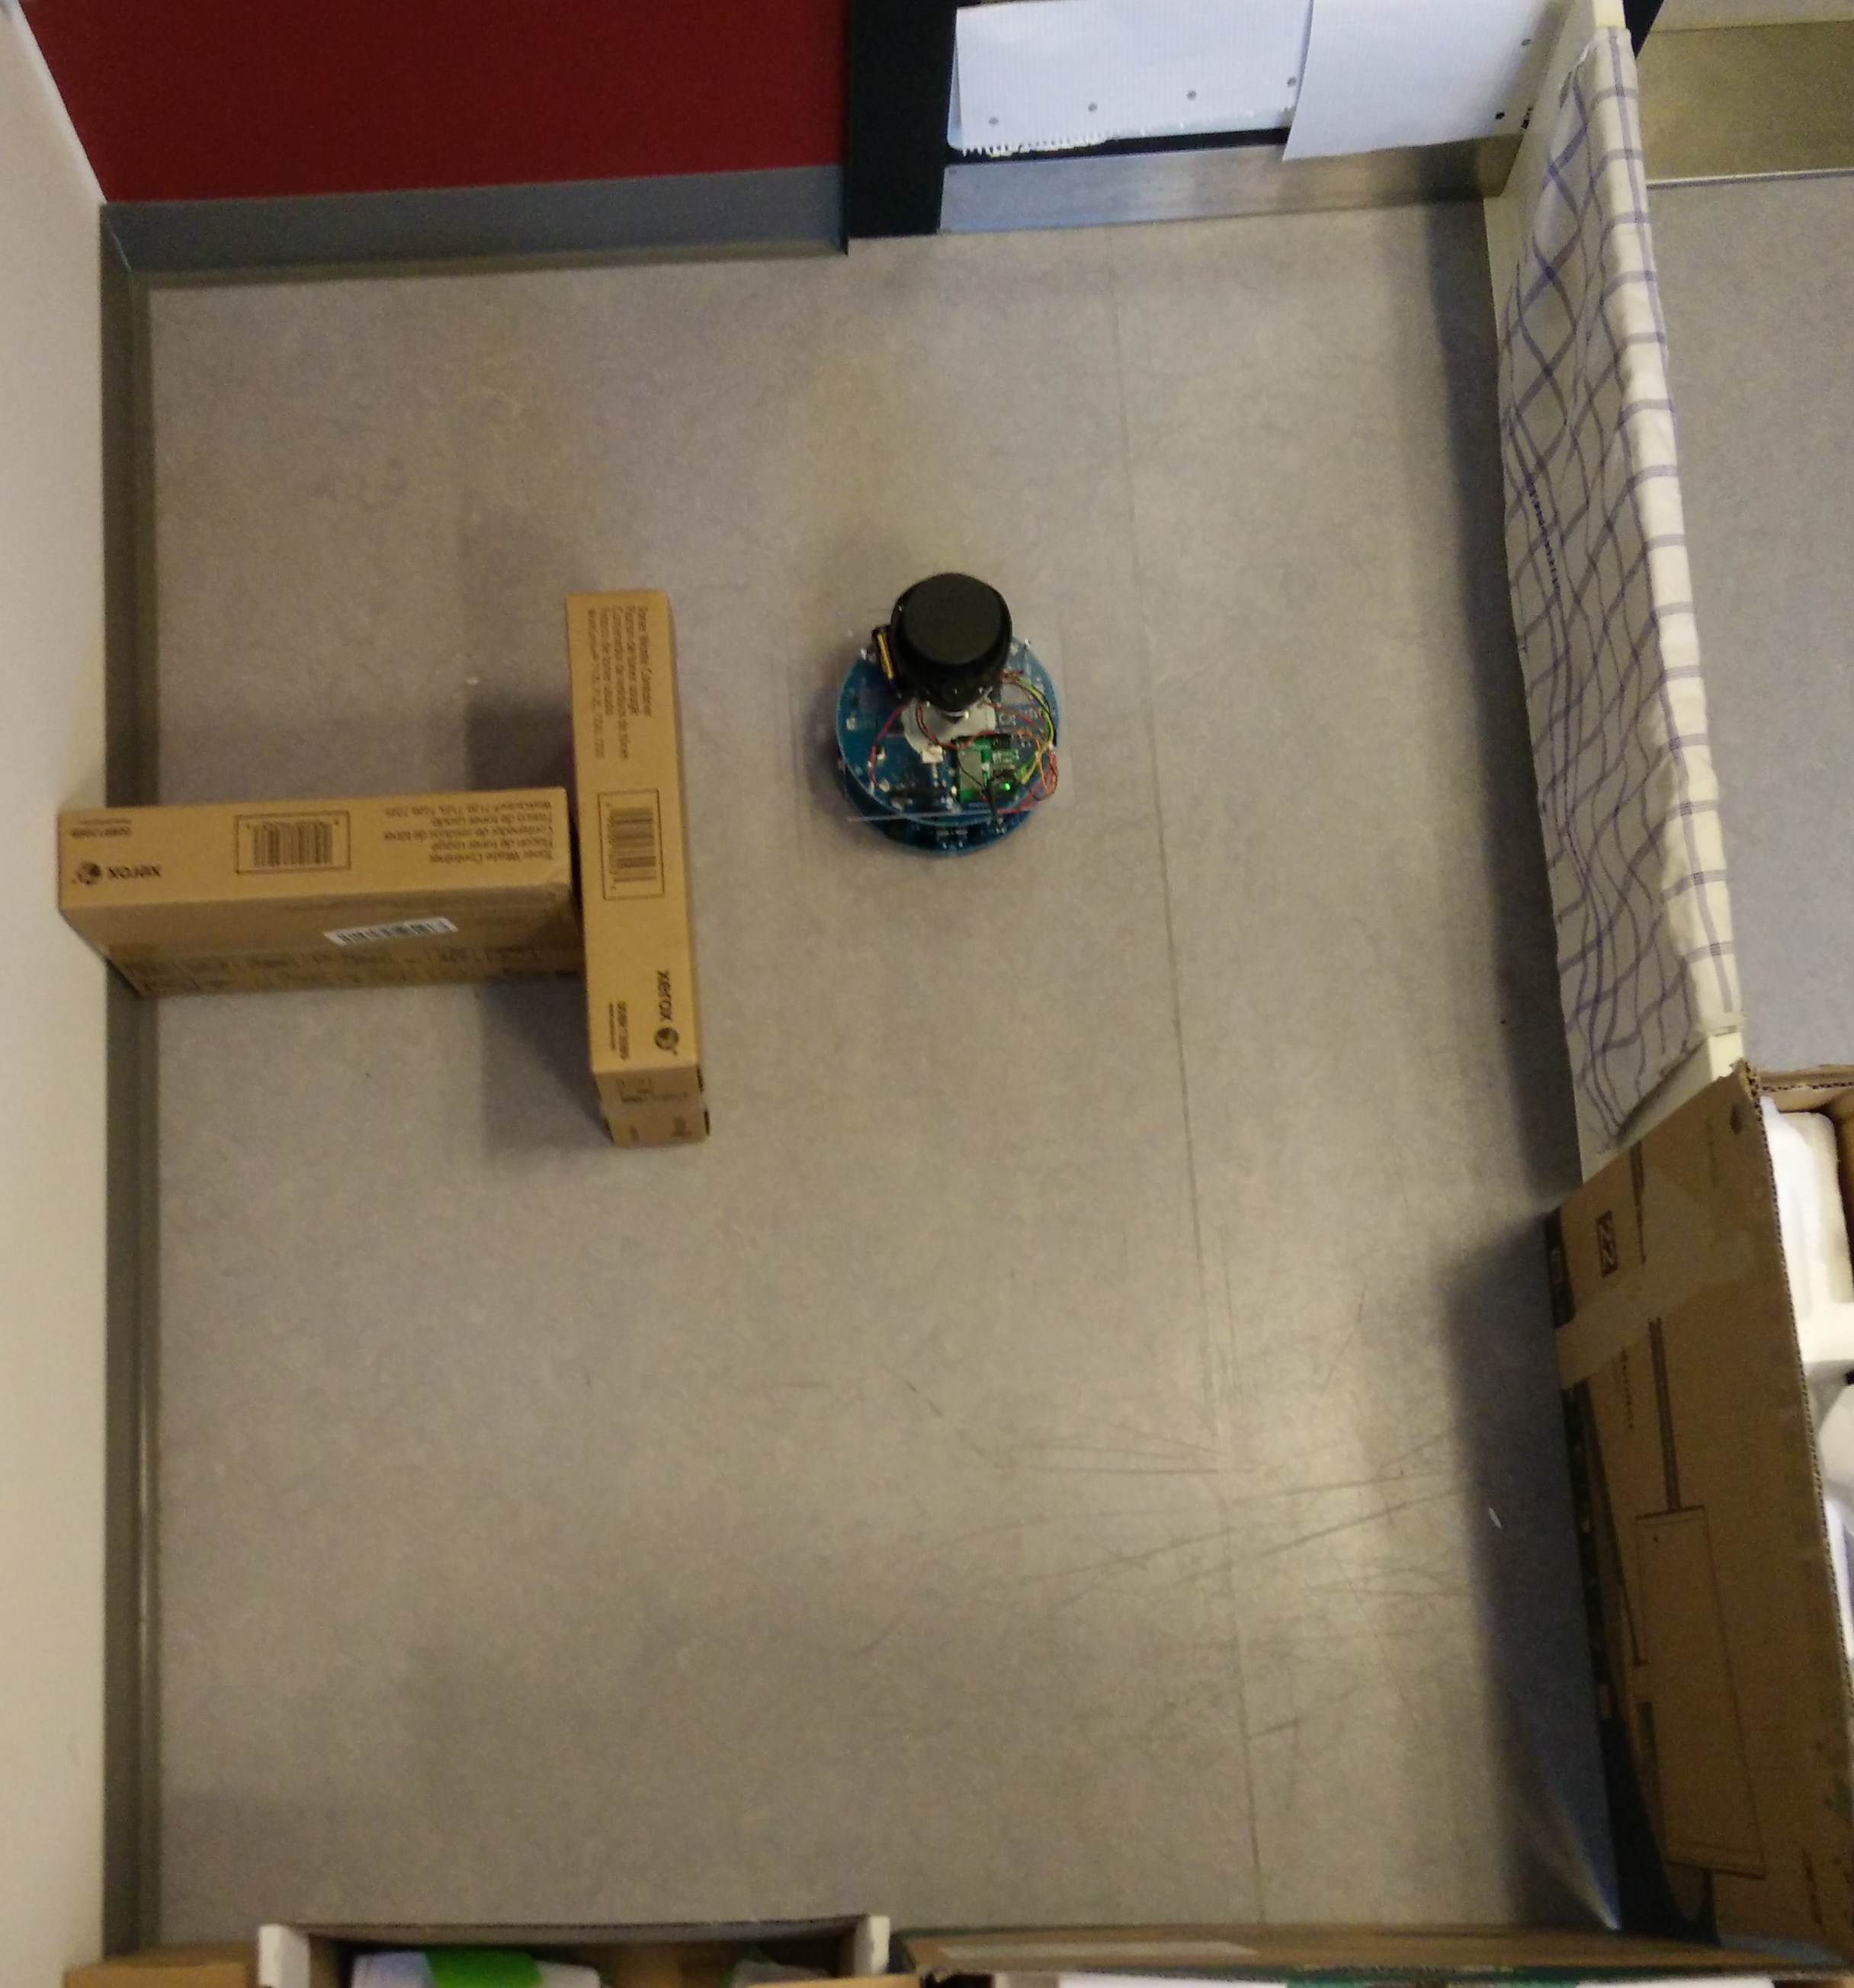
\includegraphics[width=.7\linewidth]{billeder/Results/real9.png}
  \caption{Step 9}
  \label{ResultDriveFig2:sub4}
\end{subfigure}
\begin{subfigure}{.5\textwidth}
  \centering
  \includegraphics[width=.8\linewidth]{billeder/Results/11.png}
  \caption{Step 11}
  \label{ResultDriveFig2:sub5}
\end{subfigure}%
\begin{subfigure}{.5\textwidth}
  \centering
  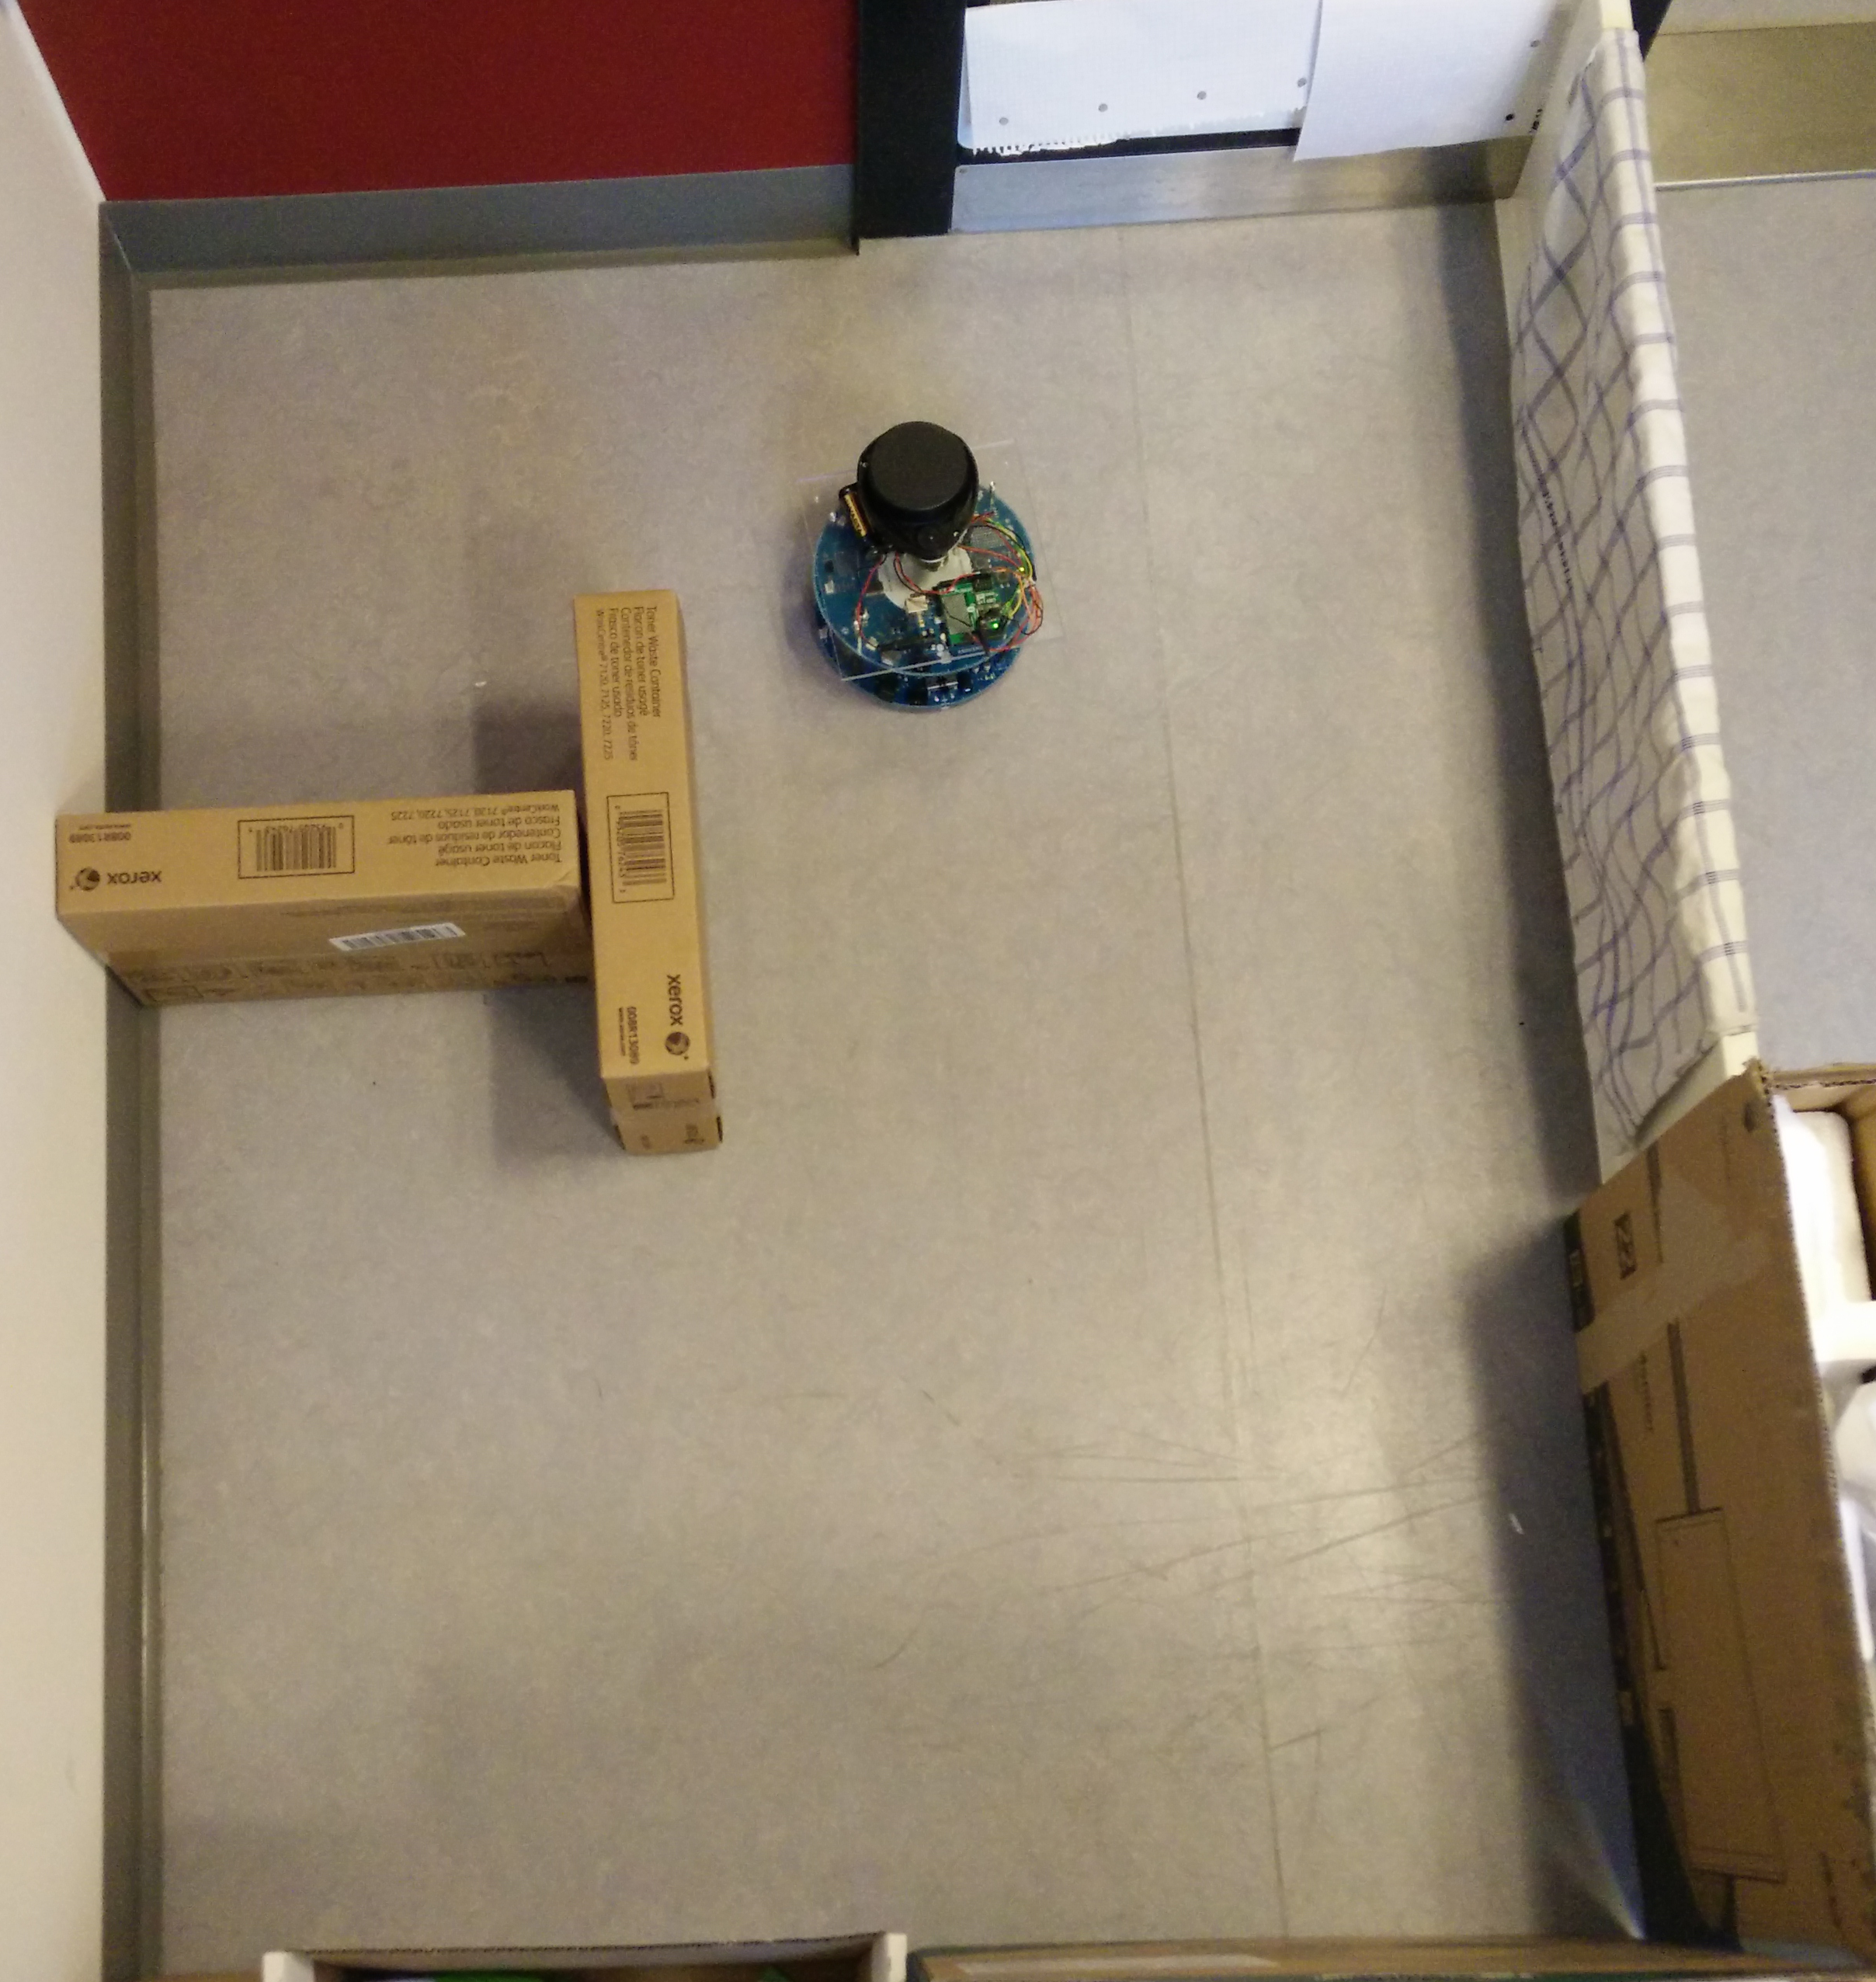
\includegraphics[width=.7\linewidth]{billeder/Results/real11.png}
  \caption{Step 11}
  \label{ResultDriveFig2:sub6}
\end{subfigure}
\caption{The robot makes a map and moves along the points on the path.}
\label{ResultDriveFig2}
\end{figure}

\begin{figure}[H]
\centering
\begin{subfigure}{.5\textwidth}
  \centering
  \includegraphics[width=.8\linewidth]{billeder/Results/13.png}
  \caption{Step 13}
  \label{ResultDriveFig3:sub1}
\end{subfigure}%
\begin{subfigure}{.5\textwidth}
  \centering
  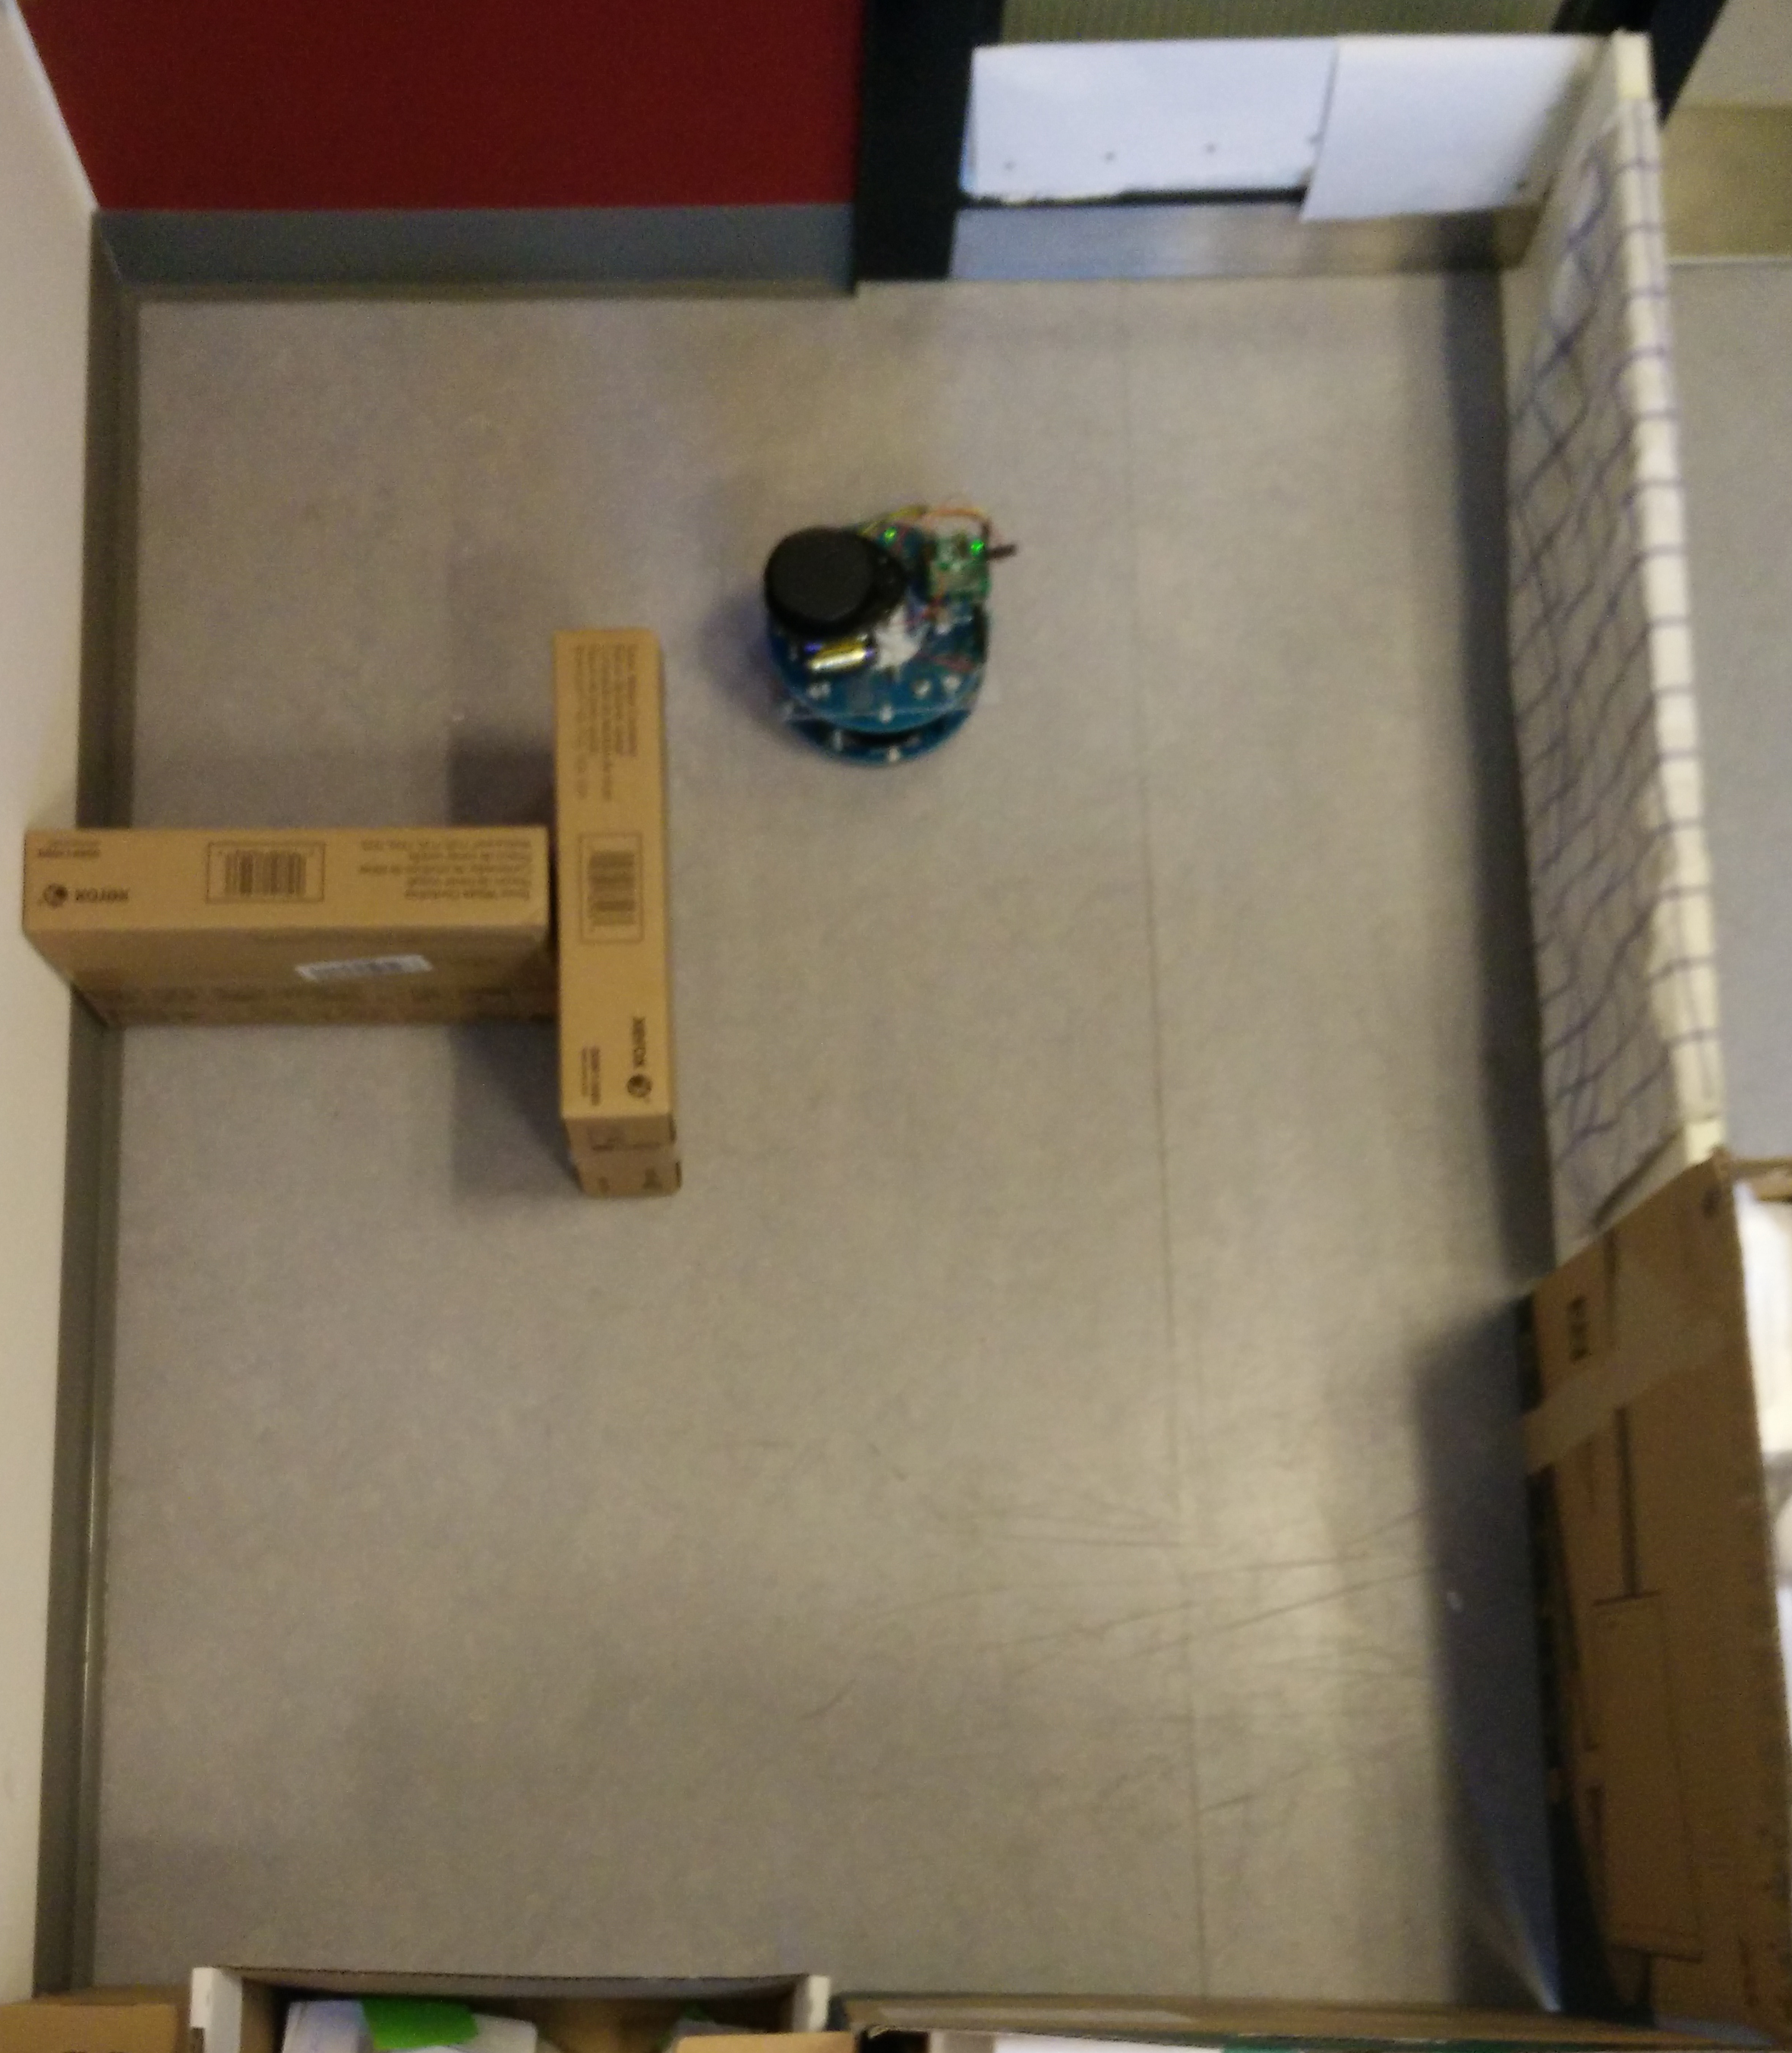
\includegraphics[width=.7\linewidth]{billeder/Results/real13.png}
  \caption{}
  \label{ResultDriveFig3:sub2}
\end{subfigure}
\begin{subfigure}{.5\textwidth}
  \centering
  \includegraphics[width=.8\linewidth]{billeder/Results/19.png}
  \caption{Step 19}
  \label{ResultDriveFig3:sub3}
\end{subfigure}%
\begin{subfigure}{.5\textwidth}
  \centering
  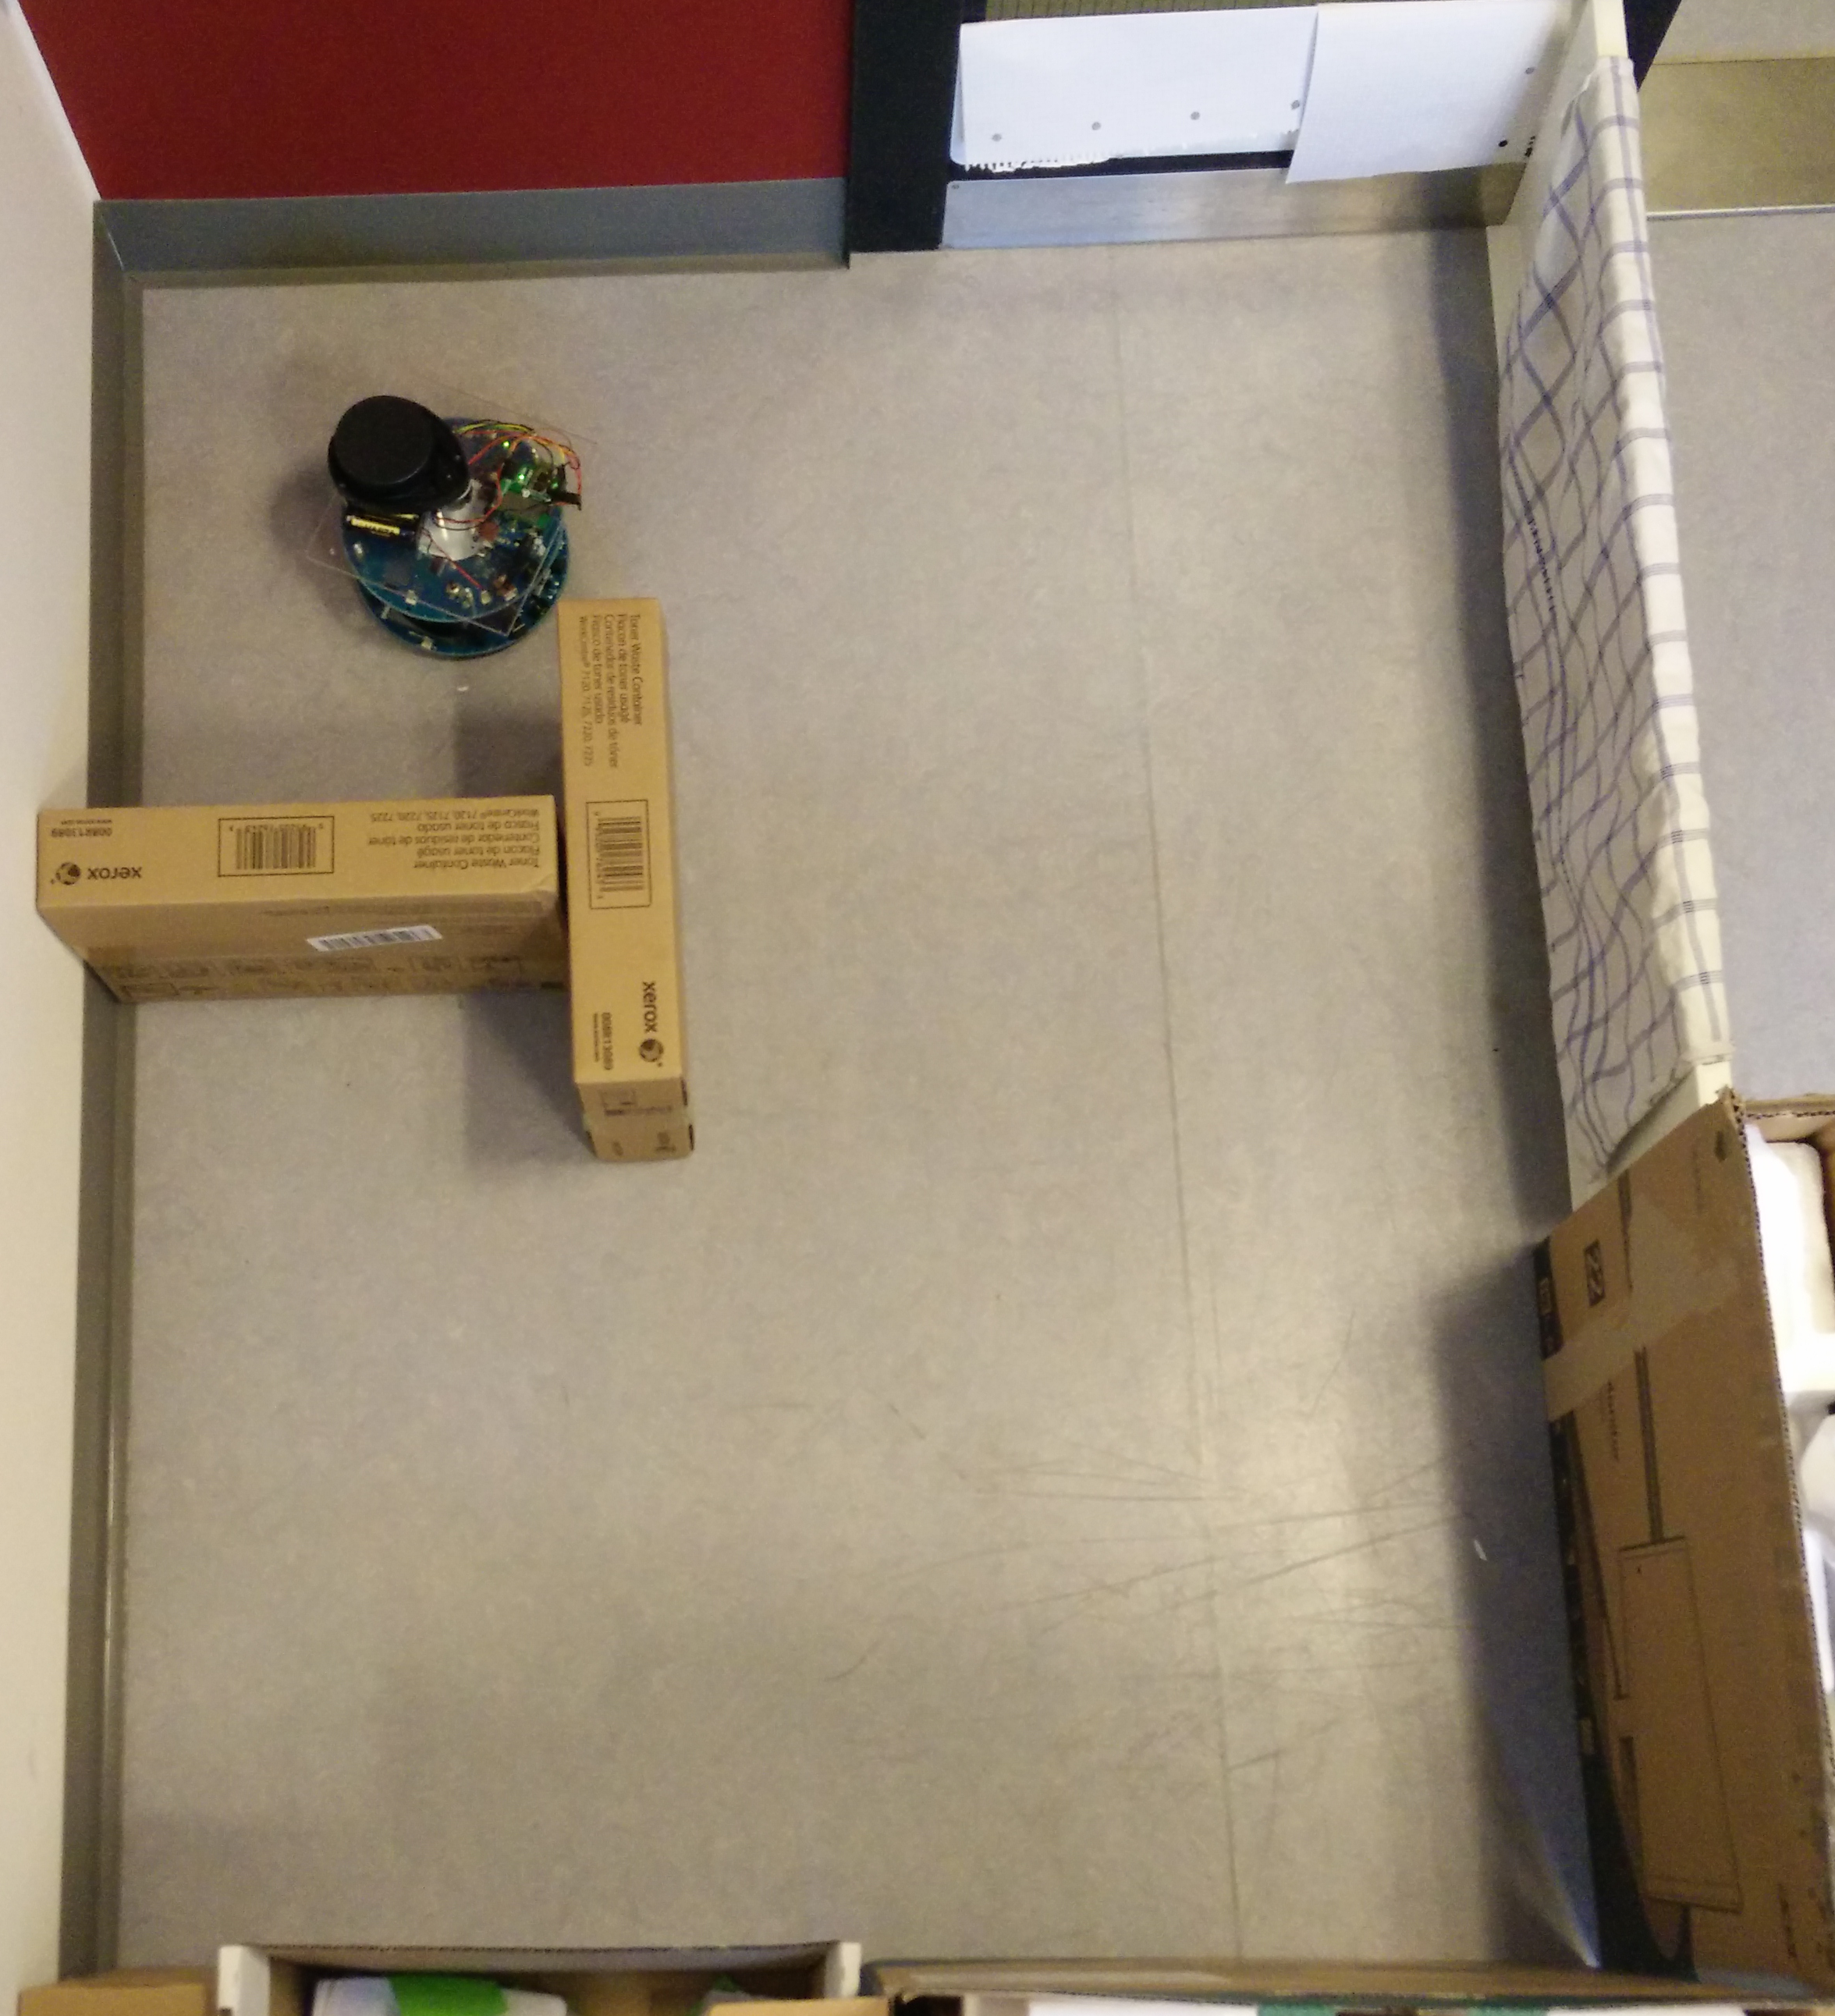
\includegraphics[width=.7\linewidth]{billeder/Results/real19.png}
  \caption{Step 19}
  \label{ResultDriveFig3:sub4}
\end{subfigure}
\begin{subfigure}{.5\textwidth}
  \centering
  \includegraphics[width=.8\linewidth]{billeder/Results/23.png}
  \caption{Step 23}
  \label{ResultDriveFig3:sub5}
\end{subfigure}%
\begin{subfigure}{.5\textwidth}
  \centering
  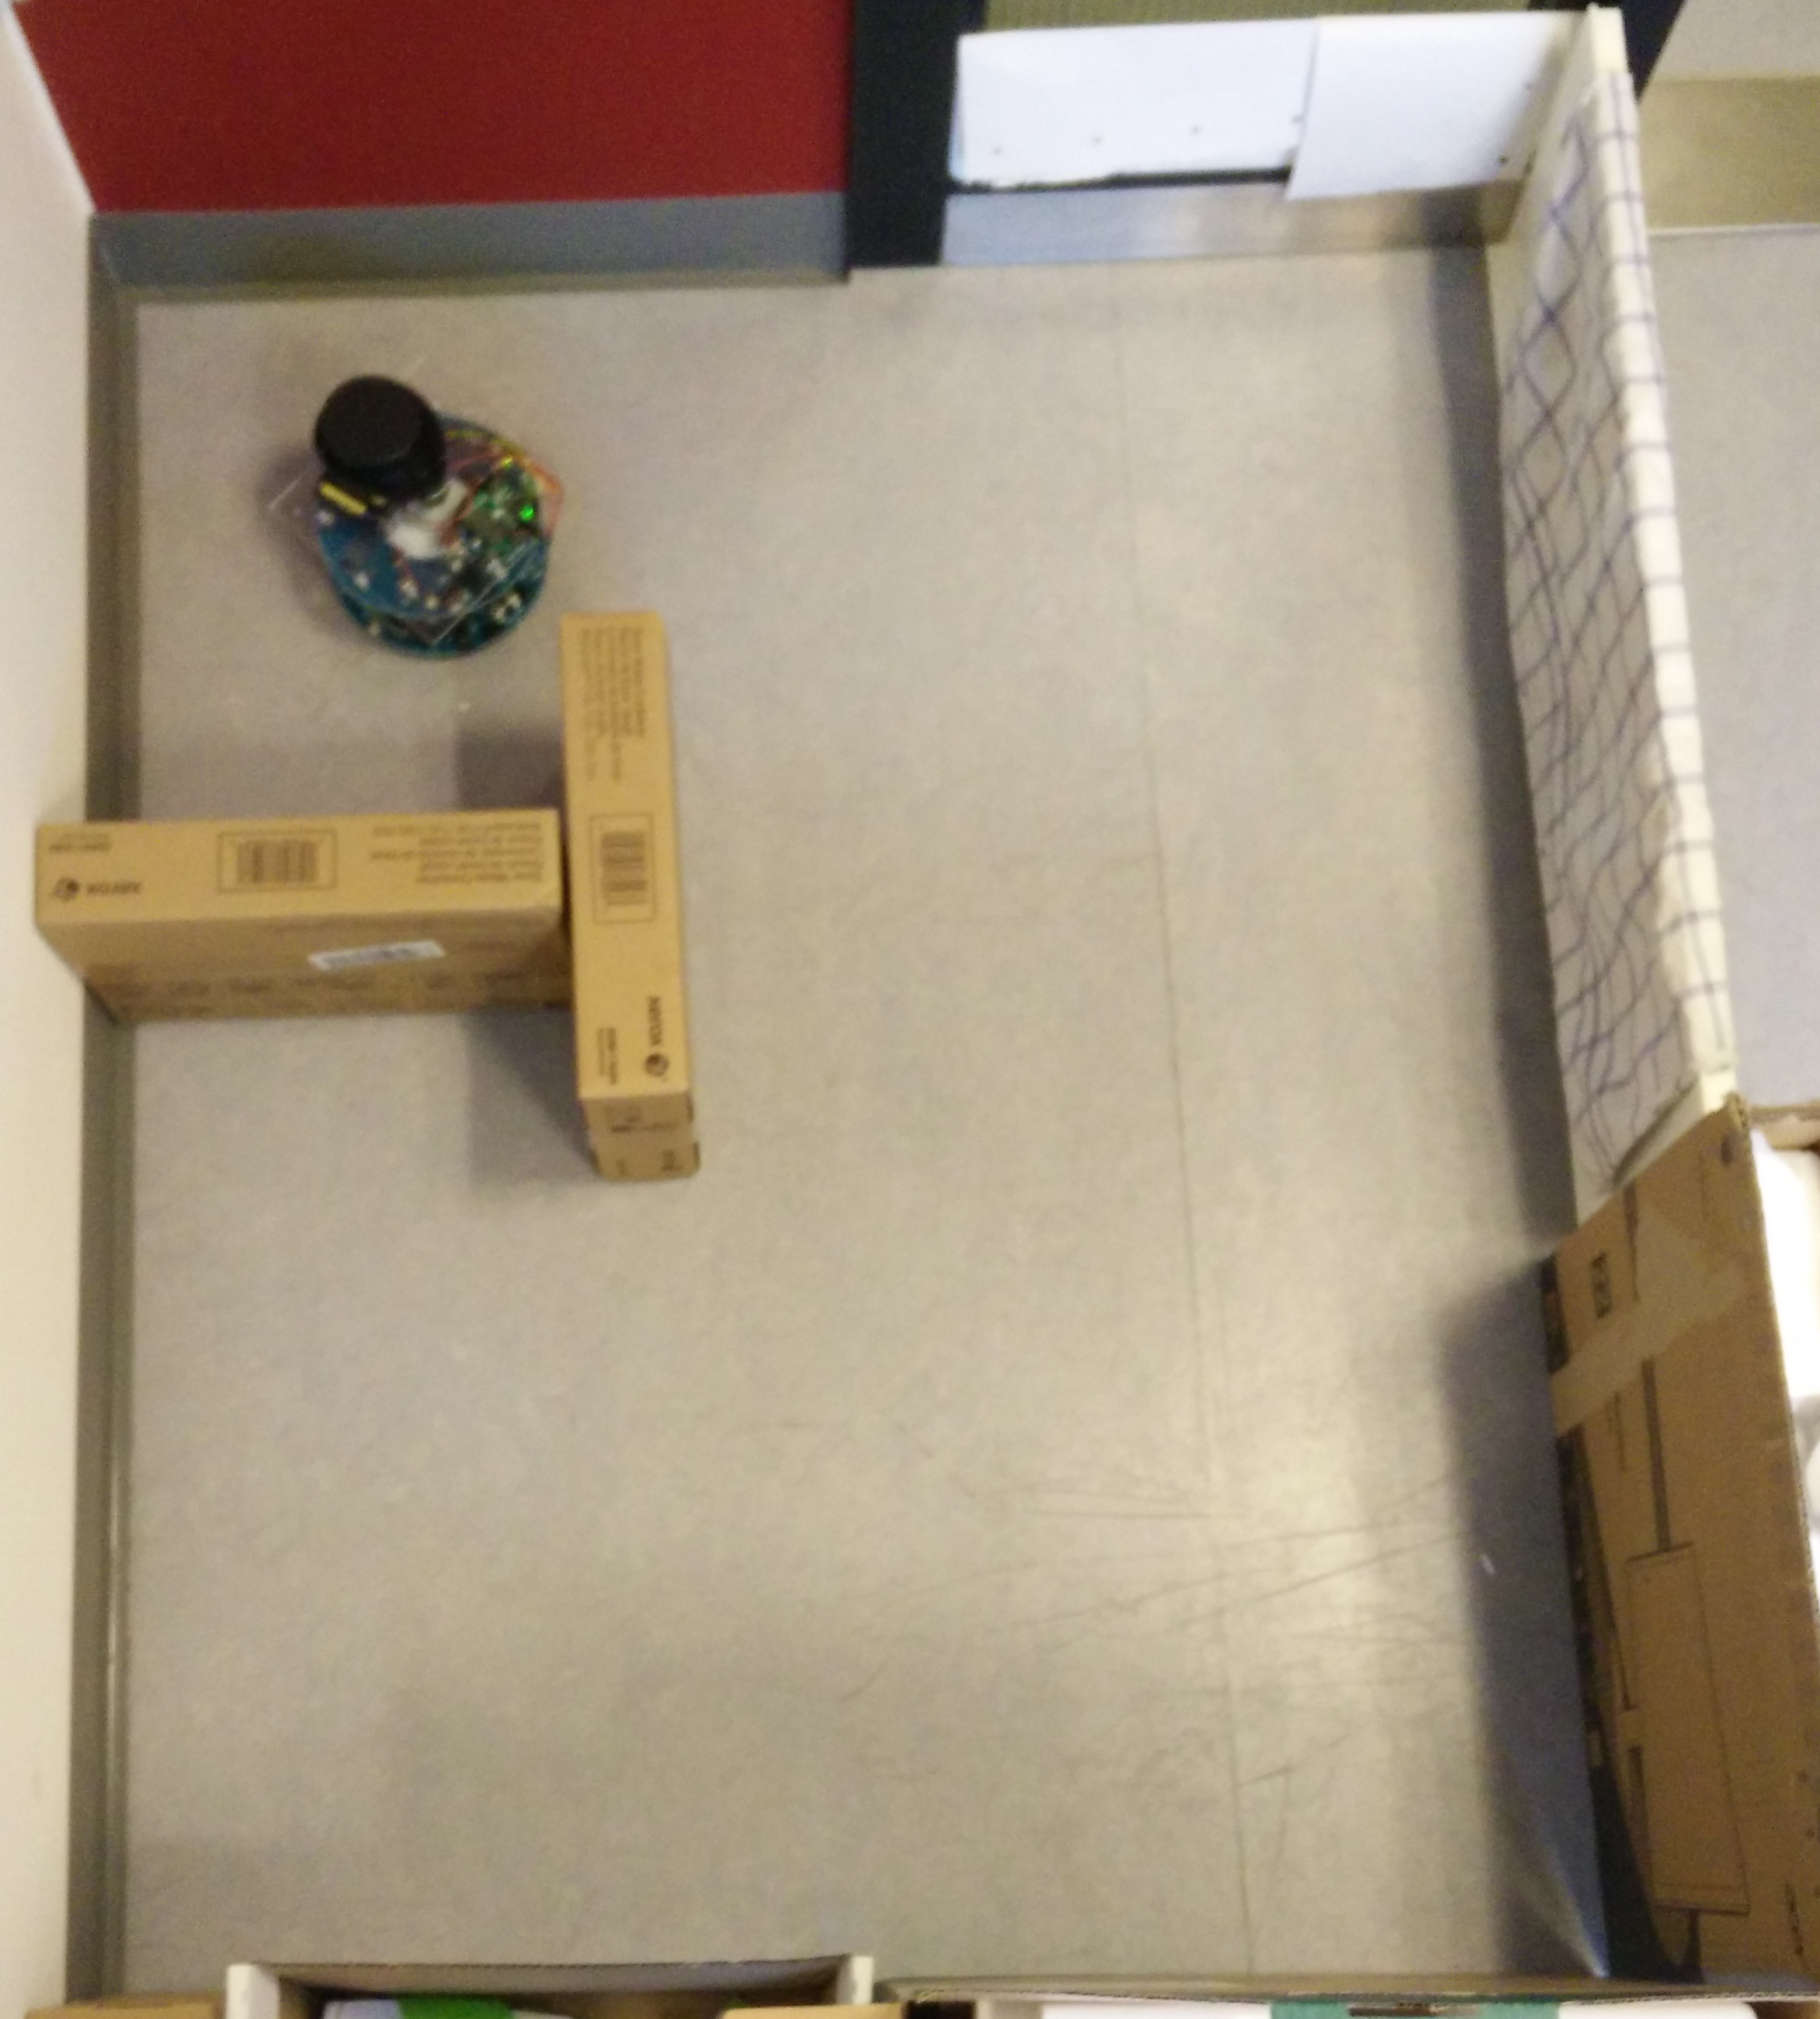
\includegraphics[width=.7\linewidth]{billeder/Results/real23.png}
  \caption{Step 23}
  \label{ResultDriveFig3:sub6}
\end{subfigure}
\caption{The robot moves along the last points of the path and reaches goal.}
\label{ResultDriveFig3}
\end{figure}

The robot used 3 steps to find it self and in total it took 23 steps from beginning to end. 

%------------------------------------------------